\documentclass[class=book, crop=false]{standalone}

%% Image paths
\usepackage{graphicx}
\graphicspath{{images/}}

%% Language and font encodings
\usepackage[english]{babel}
\usepackage[utf8x]{inputenc}
\usepackage[T1]{fontenc}

%% Sets page size and margins
\usepackage[a4paper,top=3cm,bottom=2cm,left=3cm,right=3cm,marginparwidth=1.75cm]{geometry}

%% Sets epigraph style
\usepackage{epigraph}
\setlength\epigraphwidth{.8\textwidth}
\setlength\epigraphrule{0pt}

%% Sets line style
\linespread{1.3}

%% Key term command
\usepackage{marginnote}
\providecommand{\keyterm}[1]{\textbf{#1}\marginnote{\scriptsize \textbf{#1}}}

\begin{document}

\epigraph{\itshape "Coming together is a beginning.\\Staying together is progress.\\Working together is success."}{---Henry Ford}

\section{Groupware}

Online communities frequently have to undertake joint tasks, whether it is planning events, self-moderating or just playing online video games together. It is the job of social systems to utilize whatever technological means that can aid communities in making these tasks easier to complete and more accomplish-able. There is an entire field dedicated to this task, called computer-supported cooperative work (CSCW), or groupware. Carstensen and Schmidt define the domain of CSCW as encompassing "how collaborative activities and their coordination can be supported by means of computer system" [Carstensen and Schmidt 1999].

When considering what type of groupware software to use, it is important to consider two different dimensions: time and space. Your community will use different technologies depending on whether it occupies the same physical space or is remotely located from each other. Your community will also use different technologies depending on whether members interact with each other at the same time or at different times.

Are your community members interacting in the same physical space? If so, maybe you would use a whiteboard or a large public display. Or are your community members interacting remotely? If so, maybe wikis or email would be better.

Are your community members interacting at the same time? If so, maybe you would use video conferencing or a shared table. Or are your community members interacting at different times? If so, maybe you would use project management software or group calendars.

In 1988, Johnansen created his famous time-space groupware matrix (\textbf{Figure 7.1}), which categorizes different types of interaction in a two by two matrix. By taking a quick look at the matrix, you can see what type of technology you should use to solve your problem of deciding groupware software to use.

\begin{figure}[!tbp]
  \centering
  \begin{minipage}[b]{0.8\textwidth}
    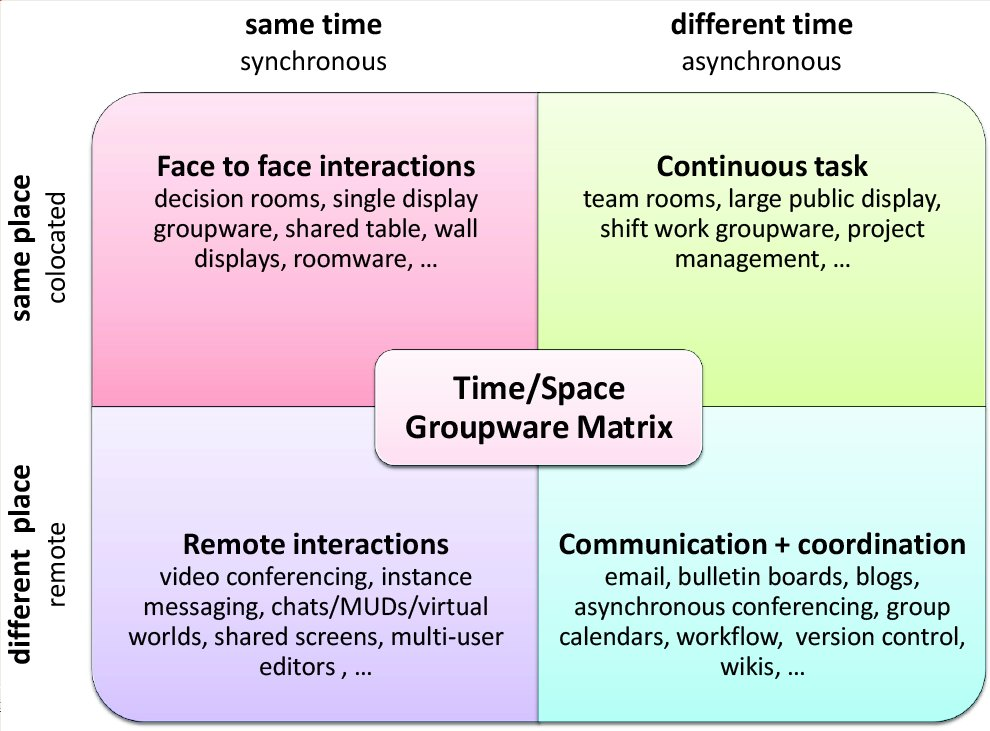
\includegraphics[width=\textwidth]{groupwarematrix}
    \caption{Johnansen's Time-Space Groupware Matrix.}
  \end{minipage}
\end{figure}

When introducing groupware software, it is also important to take into account the time and energy necessary to learn and use new groupware software. All too often, communities move to new communication platforms (Discord, Slack, GroupMe, Signal, etc.) without regard to the platforms which members are already on. This results in resistance to move to the new platforms and lack of engagement with the new platforms, as users now have to deal with yet another communication platform (I have over eight messaging apps on my phone alone -- at some point, this is really too much!). Even if a new communication platform seems optimal for your goals, take into account whether the benefits of moving to the new communication platform outweigh the possibility and the costs of users having to operate yet another communication platform.

\section{Social translucence}

When interacting or collaborating with others online, it is of paramount importance to be kept aware of what others are doing online. This is the concept of \keyterm{social translucence}, or social awareness, which is described by its creators Thomas Erickson and Wendy Kellogg as "digital systems that support coherent behavior by making participants and their activities visible to one another" [Erickson and Kellogg 2000].

In real life, you are continuously aware of what your nearby friends and colleagues are doing. You can see if your work neighbor is in his or her office or not. You pass by your colleagues on the way to the bathroom and overhear them talking about the new feature they're adding and it sounds interesting. You observe your friends playing catch outside and decide to go join them. You see that a lot of shoppers are hovering around the new computer and decide to go check it out. All these events are happening, whether you set out to observe them or not, and you are kept peripherally aware of them. This peripheral awareness is what allows you to learn of that one interesting work project or find out that your friends are playing catch. One of the biggest problems of social translucence thus becomes, how do we keep online community members continuously aware of what others are doing online?

Erickson and Kellogg define three principles of socially translucent systems: visibility, awareness and accountability [Erickson and Kellogg 2000]. A system promotes visibility if users are able to see helpful or relevant information. A system promotes awareness if users are guided to notice the information (there are lots of ways to accomplish this, from using headers to effective use of whitespace). A system promotes accountability if users are held responsible for the effects of their actions. For example, if a user defaces a wiki page, they are held accountable if there is a view-able record of who defaced the page.

\section{Grudin's paradox}

In 1988, Jonathan Grudin conceptualized a famous problem, which is commonly known as \keyterm{Grudin's paradox}, or Grudin's problem. The problem essentially states that in a corporation, the people who work on a product and the people who benefit from the product (i.e. the manager or the owners) are not the same. Consequently, if their interests do not align, then the interests of the people who work on a product will likely win out and the interests of the manager or owners will not be followed. [Grudin 1988]

In his paper, Grudin uses organizational use of electronic calendars as an example of Grudin's paradox. Many electronic calendars have an automatic meeting scheduling feature, which essentially looks at all the calendars of everybody signed up for a meeting and finds meeting times which work for everybody. This necessarily requires that everybody in the organization keep their calendars updated, a requirement which does not often play out. Though it is in the manager's best interest to update their calendar, as they are in charge of running meetings and checking in with all team members, it is not in the workers' best interest, as they would likely not otherwise use the calendars. Consequently, when managers try to make everybody update their calendars, they rarely do so, and this feature fails.

\section{Reading questions}

\section{Solutions to reading questions}

\section{Bibliography}

Carstensen, P. H. and Schmidt, K. "Computer supported cooperative work: new challenges to systems design." 1999.

Dabbish, Laura et al. "Social coding in GitHub: transparency and collaboration in an open software repository." Proceedings of the ACM 2012 conference on Computer Supported Cooperative Work. pp. 1277-1286. February 11 - 15, 2012.

Erickson, Thomas and Kellogg, Wendy. "Social transluence: an approach to designing systems that support social processes." ACM Transactions on Computer-Human Interaction. 7 (1): 59-83. March 1, 2000.

Godwin-Jones, Robert. "Emerging Technologies: Blogs and Wikis: Environments for On-line Collaboration." Language Learning \& Technology 7 (2): pp. 12-16. May, 2003.

Grudin, Jonathan. "Groupware and Social Dynamics: Eight Challenges for Developers." Communications of the ACM. 37.1. January, 1994.

Grudin, Jonathan and Poole, Erika Shehan. "Wikis at Work: Success Factors and Challenges for Sustainability of Enterprise Wikis." WikiSym 2010. July 7 - 9, 2010.

Grudin, Jonathan. "Why CSCW Applicatoins Fail: Problems in the Design and Evaluation of Organizational Interfaces." ACM. 1988.

\end{document}
